\documentclass[./project-report/src/latex/project-report.tex]{subfiles}

\begin{document}

\maketitle

\section{Design}

\subsection{Introduction}

The following design focuses have been made for the project:

\begin{itemize}
    \item The program will support multiple platforms to run on, including Windows and Linux.
    \item The program will use python3 as its main programming language.
    \item I will take an object-orientated approach to the project.
    \item I will give an option to use either a Graphics Card or a CPU to train the Artificial Neural Networks.
\end{itemize}

I will also be using SysML for designing the following diagrams.

\subsection{System Architecture}

\begin{figure}[h!]
\centering
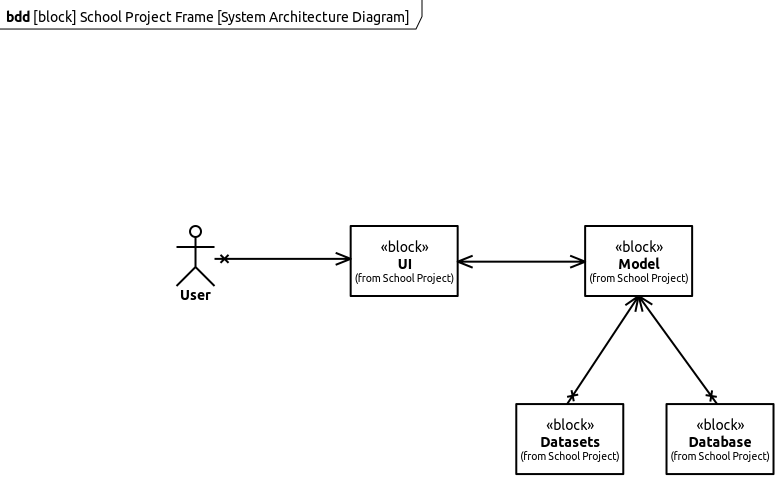
\includegraphics[width=1\textwidth]{./project-report/src/images/system-architecture-diagram.png}
\end{figure}

\pagebreak

\subsection{Class Diagrams}

\subsubsection{UI Class Diagram}

\begin{figure}[h!]
\centering
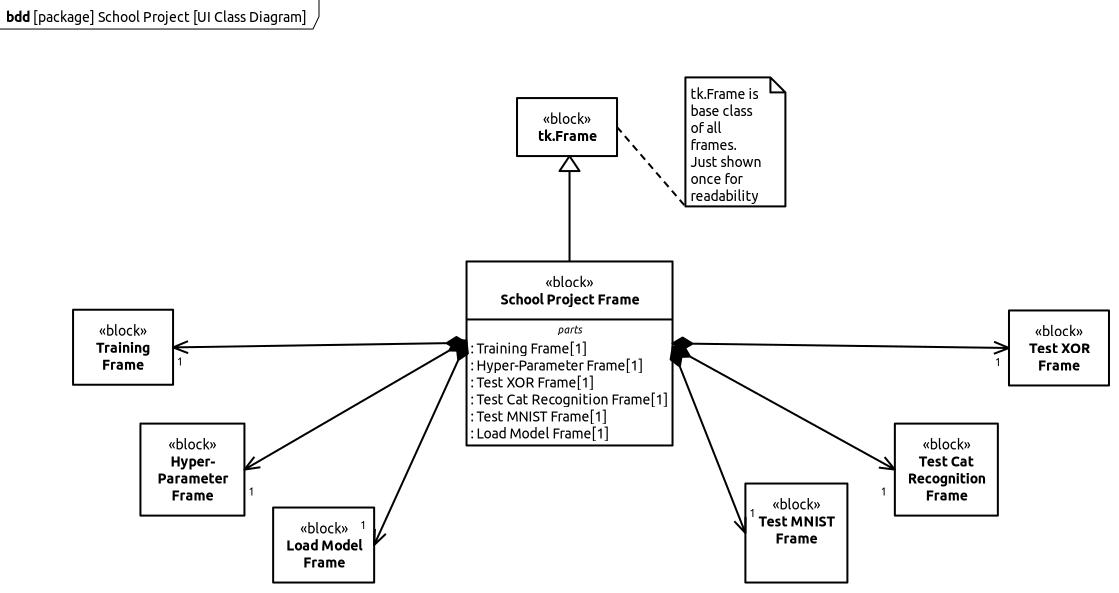
\includegraphics[width=1\textwidth]{./project-report/src/images/ui-class-diagram.png}
\end{figure}

\subsubsection{Model Class Diagram}

\begin{figure}[h!]
\centering
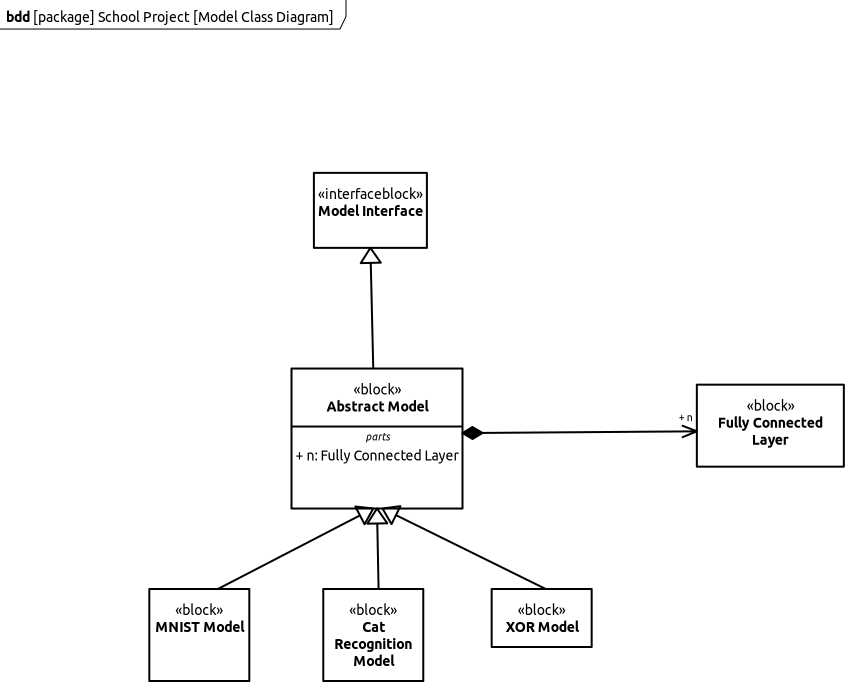
\includegraphics[width=1\textwidth]{./project-report/src/images/model-class-diagram.png}
\end{figure}

\pagebreak

\subsection{System Flow chart}

\begin{figure}[h!]
\centering
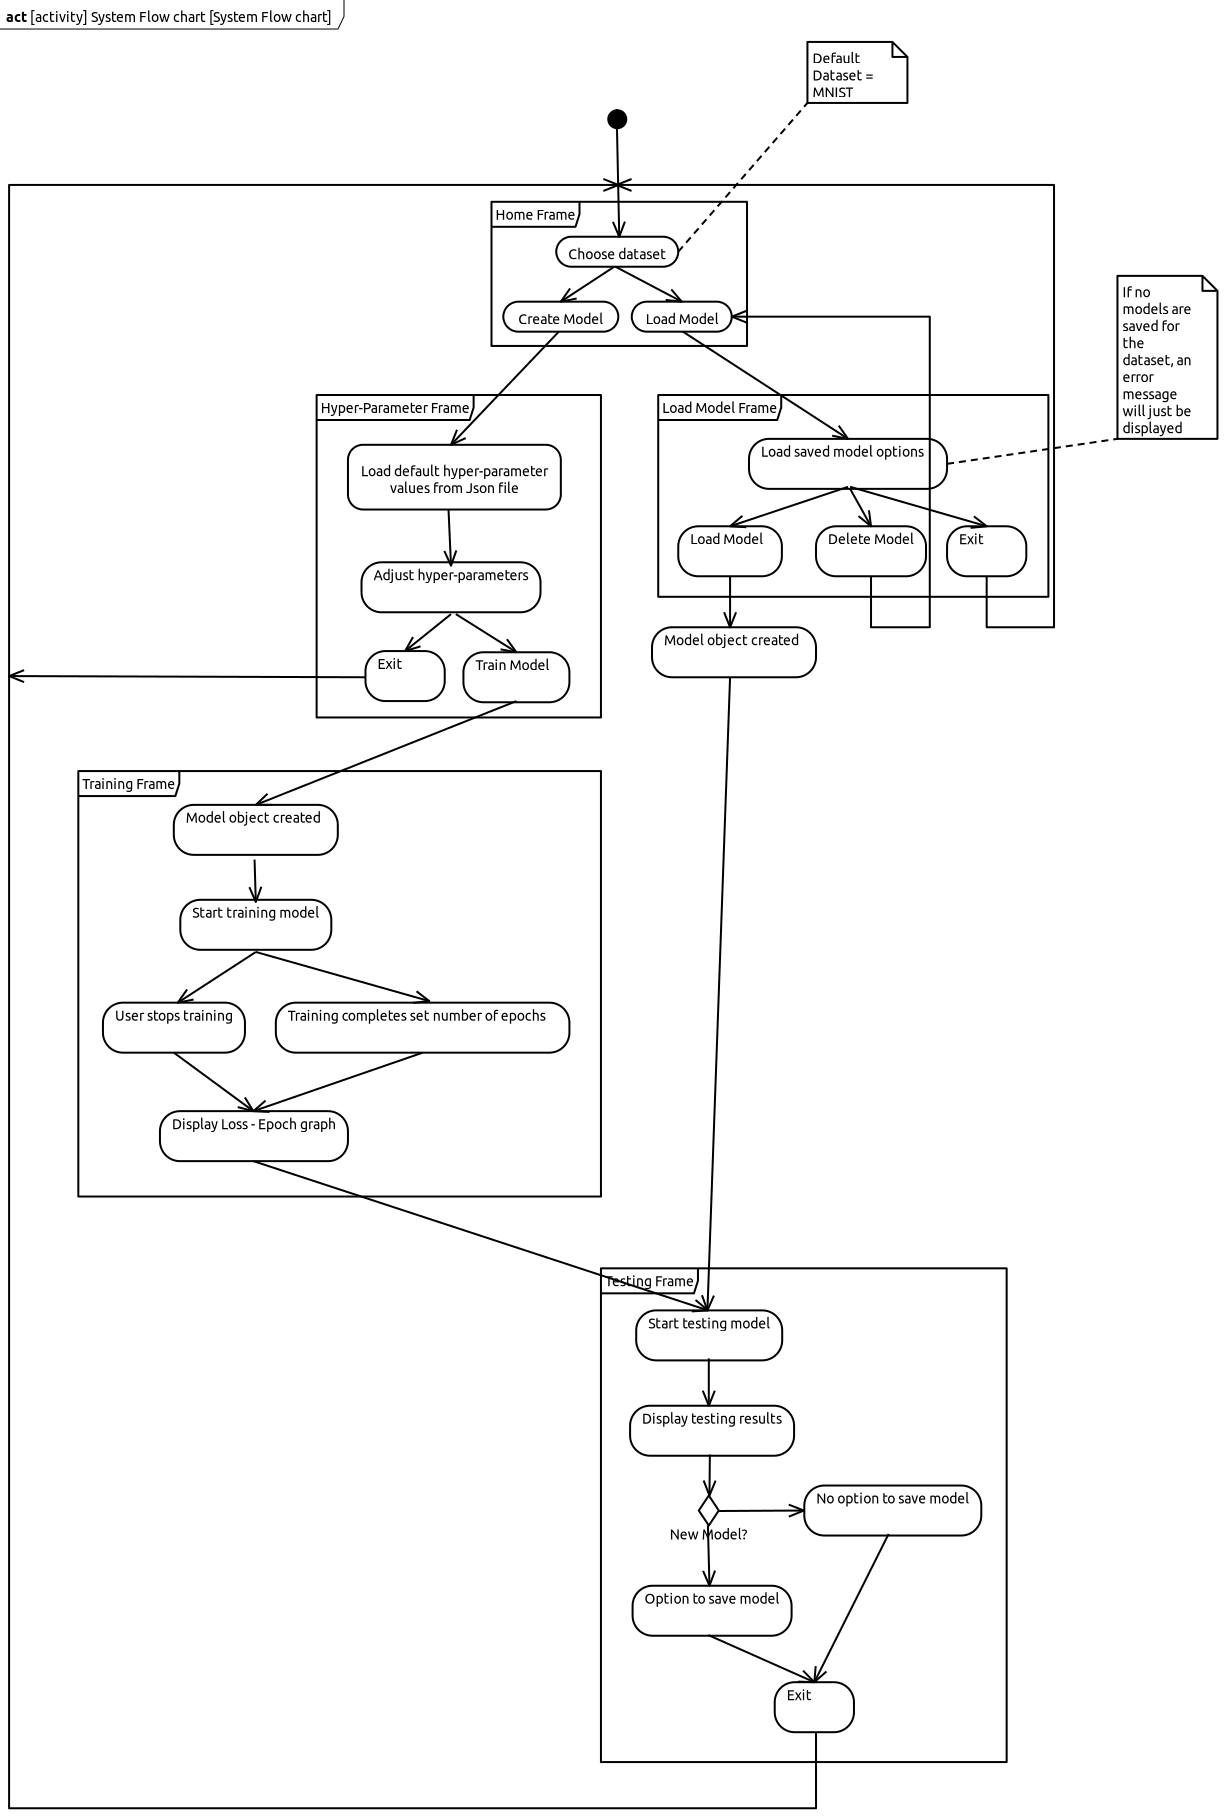
\includegraphics[width=1\textwidth]{./project-report/src/images/system-flow-chart.png}
\end{figure}

\subsection{Algorithms}

Refer to Analysis for the algorithms behind the Artificial Neural Networks.

\subsection{Data Structures}

I will use the following data structures in the program:

\begin{itemize}
    \item Standard arrays for storing data contiguously, for example storing the shape of the Artificial Neural Network's layers.
    \item Tuples where tuple unpacking is usefull, such as returning multiple values from methods.
    \item Dictionaries for loading the default hyper-parameter values from a JSON file.
    \item Matrices to represent the layers and allow for a varied number of neurons in each layer. To represent the Matrices I will use both numpy arrays and cupy 
          arrays.
    \item A Doubly linked list to represent the Artificial Neural Network, where each node is a layer of the network. This will allow me to traverse both forwards and 
          backwards through the network, as well as storing the first and last layer to start forward and backward propagation respectively.
\end{itemize}

\subsection{File Structure}

I will use the following file structures to store necessary data for the program:

\begin{itemize}
    \item A JSON file for storing the default hyper-parameters for creating a new model for each dataset.
    \item I will store the image dataset files in a 'datasets' directory. The dataset files will either be a compressed archive file (such as .pkl.gz files) or of the 
          Hierarchical Data Format (such as .h5) for storing large datasets with fast retrieval.
    \item I will save the weights and biases of saved models as numpy arrays in .npz files (a zipped archive file format) in a 'saved-models' directory, due to 
          their compatibility with the numpy library.
\end{itemize}

\pagebreak

\subsection{Database Design}

I will use the following Relational database design for saving models, where the dataset, name and features of the saved model (including the location of the 
saved models' weights and biases and the saved models' hyper-parameters) are saved:

\begin{figure}[h!]
\centering
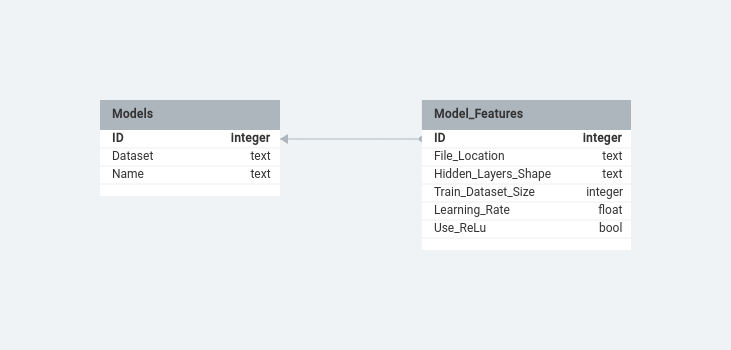
\includegraphics[width=1\textwidth]{./project-report/src/images/database-design.png}
\end{figure}

\subsection{Queries}

Here are some example queries for interacting with the database:

\begin{itemize}
    \item I can query the names of all saved models for a dataset with:
    \begin{minted}{sql}
    SELECT Name FROM Models WHERE Dataset=?;
    \end{minted}
    \item I can query the ID of a saved model for a dataset with:
    \begin{minted}{sql}
    SELECT ID FROM Models WHERE Dataset=? AND Name=?;
    \end{minted}
    \item I can query the file location of a saved model with:
    \begin{minted}{sql}
    SELECT File_Location FROM Model_Features WHERE ID=?;
    \end{minted}
    \item I can query the features of a saved model with:
    \begin{minted}{sql}
    SELECT * FROM Model_Features WHERE ID=?;
    \end{minted}
\end{itemize}

\subsection{Human-Computer Interaction TODO}

- Labeled screenshots of UI

\subsection{Hardware Design}

To allow for faster training of an Artificial Neural Network, I will give the option to use a Graphics Card to train the Artificial Neural Network if available. 
I will also give the option to load pretrained weights to run on less computationaly powerfull hardware using just the CPU as standard.

\end{document}